\section{Plasma Nanotechnology}

\begin{frame} {Plasma Nanotechnology}
    Nanotechnology:
    \begin{itemize}
        \item Manipulation of matter with size of nanometers to create materials.
        \item Synthesis is the most active areas of research.
    \end{itemize}

    Plasma nanotechnology:
    \begin{itemize}
        \item Utilizes plasma to synthesize materials.
        \item Plasma Based and plasma-assisted process provide a complex, reactive and far from equilibrium chemical factory.
    \end{itemize}
\end{frame}

\begin{frame} {Classification of Plasmas in Plasma Nanotechnology}
    \begin{itemize}
        \item low temperature
              (cold) plasmas which are used by industry and material research community
        \item high temperature
              (hot) high energy density plasmas from fusion, pinch and intense discharge sources with densities and
              temperatures many orders of magnitude higher than that of cold plasmas
    \end{itemize}
    \begin{figure}
        \centering
        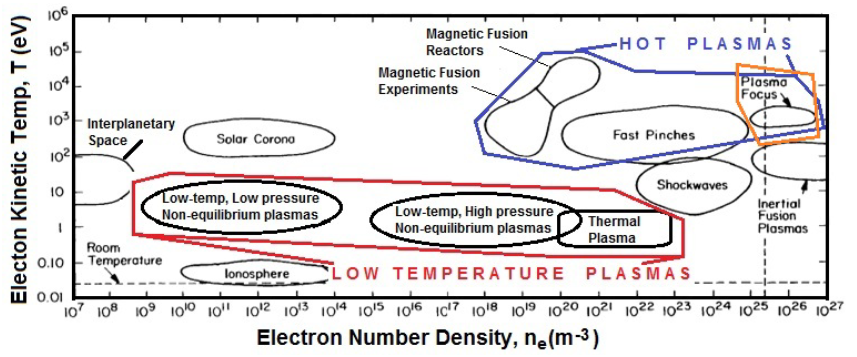
\includegraphics[width=0.7\textwidth]{figures/plasma-classification.png}
        \caption{\scriptsize The plasma parameters of various types of plasmas. The low temperature plasmas routinely used in plasma nanotechnology are inside the red box while the high energy density DPF source is shown orange and blue box which belong to the category of hot plasmas. \cite{rawat_2015_dense}}
        \label{fig:plasma-classification}
    \end{figure}
    \tiny{\cite{rawat_2015_dense} R. S. Rawat. Dense plasma focus - from alternative fusion source to versatile high energy density plasma source for plasma nanotechnology.}
\end{frame}

\begin{frame} {Low Temperature (Cold) Plasmas for Plasma Nanotechnology}
    \begin{itemize}
        \item Mainly produced by ac or dc electric gas discharge or by gas discharges initiated by RF or microwave electromagnetic fields.
        \item Electron kinetic temperature: fractions to few tens of eV with low degree of gas ionization.
    \end{itemize}

    The non-equilibrium plasmas are formed when either
    \begin{itemize}
        \item The low operating pressure results in insufficient collisions between electrons and ions and neutrals
        \item Or high operating pressure having higher collision rates but the plasmas are short lived interrupting the equilibration process.
    \end{itemize}

    The thermal plasmas are
    \begin{itemize}
        \item The plasmas in thermal equilibrium
              where the frequent collision between the electrons and ions and neutrals results in equilibration of temperatures among the charged and neutral species.
    \end{itemize}
\end{frame}

\begin{frame} {High Energy Density High Temperature (Hot) Plasmas for Plasma Nanotechnology}
    \begin{itemize}
        \item Have temperatures from few to several keV.
        \item Almost fully-ionized.
        \item DPF device is able to make such plasmas.
    \end{itemize}
\end{frame}

\begin{frame} {DPF: Device Layout, Plasma Dynamics and Key Features}
    \begin{figure}
        \centering
        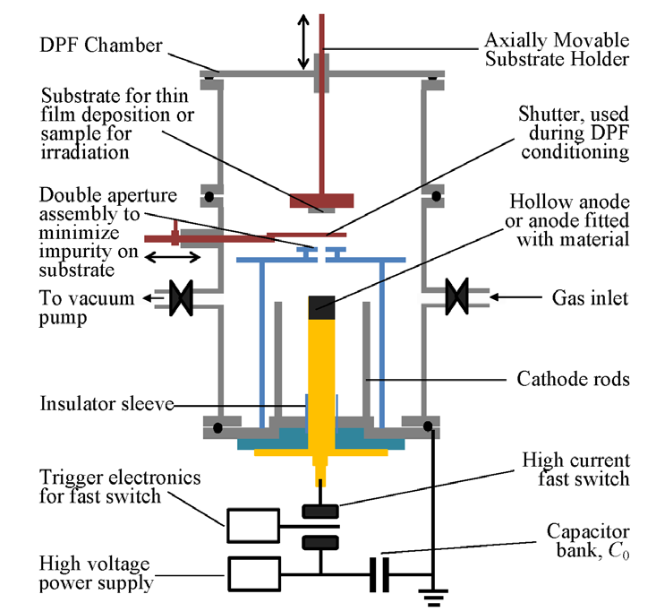
\includegraphics[width=0.5\textwidth]{figures/dpf-device-layout.png}
        \caption{The schematic of DPF material processing/synthesis facility with its various subsystems. \cite{rawat_2015_dense}}
        \label{fig:dpf-device-layout}
    \end{figure}
    \tiny{\cite{rawat_2015_dense} R. S. Rawat. Dense plasma focus - from alternative fusion source to versatile high energy density plasma source for plasma nanotechnology.}
\end{frame}

\begin{frame} {Top-down and Bottom-up Nanoscale Fabrications using DPF devices.}
    \begin{itemize}
        \item Bottom-up: Creates nanoscale materials from assembling atoms and molecule.
        \item Top-down: Relies on the successive fragmentations or processing of macro-scale materials to smaller nano-sized objects.
    \end{itemize}
    \begin{figure}
        \centering
        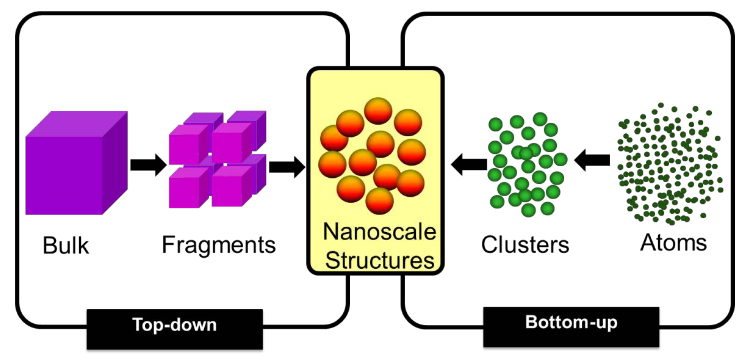
\includegraphics[width=0.7\textwidth]{figures/top-down-vs-bottom-up.png}
        \caption{"Top-down" and "bottom-up" synthesis of nanofabrication.}
        \label{fig:top-down-vs-bottom-up}
    \end{figure}
    \tiny{\cite{rawat_2015_dense} R. S. Rawat. Dense plasma focus - from alternative fusion source to versatile high energy density plasma source for plasma nanotechnology.}
\end{frame}

\begin{frame} {Top-down Nanoscale Fabrication by Transient Processing of Bulk/Thin Films in DPF}
    \begin{itemize}
        \item Involves the exposure of bulk or thin film samples to the different number of DPF shots.
        \item Nanostructurization of the entire thickness of the thin film can be achieved by its exposure to DPF shots.
        \item For bulk material only the top surface layer of the bulk sample is processed and nanostructurized by its exposure to DPF shots.
    \end{itemize}
\end{frame}

\begin{frame} {SEM Images of Unexposed and Irradiated Ti and W samples in Different DPF Devices}
    \begin{figure}
        \centering
        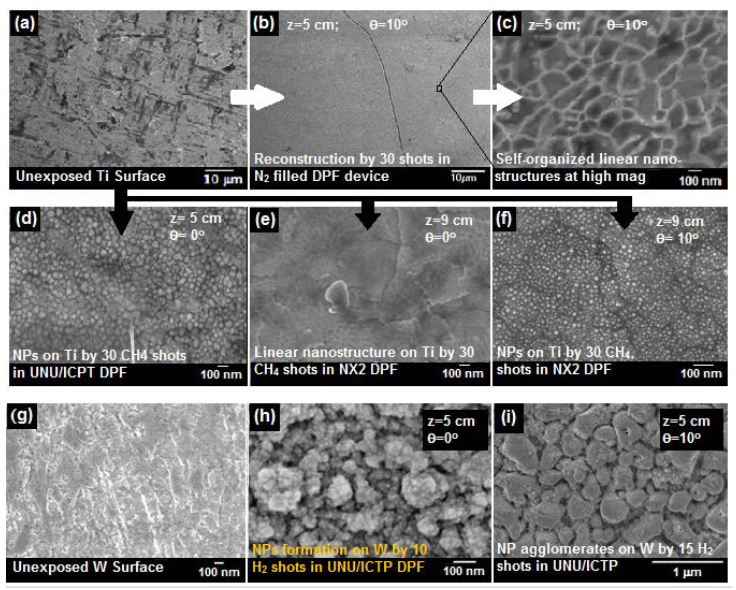
\includegraphics[width=0.5\textwidth]{figures/irradiated-ti-and-w-samples.png}
        \caption{\scriptsize SEM images of unexposed and irradiated Ti and W samples in different DPF devices. The distance ($z$) and angular position ($\theta$) of the samples, number of DPF irradiation shots and DPF operating gas for each of the exposure experiment are mentioned in SEM images. \cite{rawat_2015_dense}}
        \label{fig:irradiated-ti-and-w-samples}
    \end{figure}
    \tiny{\cite{rawat_2015_dense} R. S. Rawat. Dense plasma focus - from alternative fusion source to versatile high energy density plasma source for plasma nanotechnology.}
\end{frame}

\begin{frame} {Combined Schematic of DPF Device}
    \begin{figure}
        \centering
        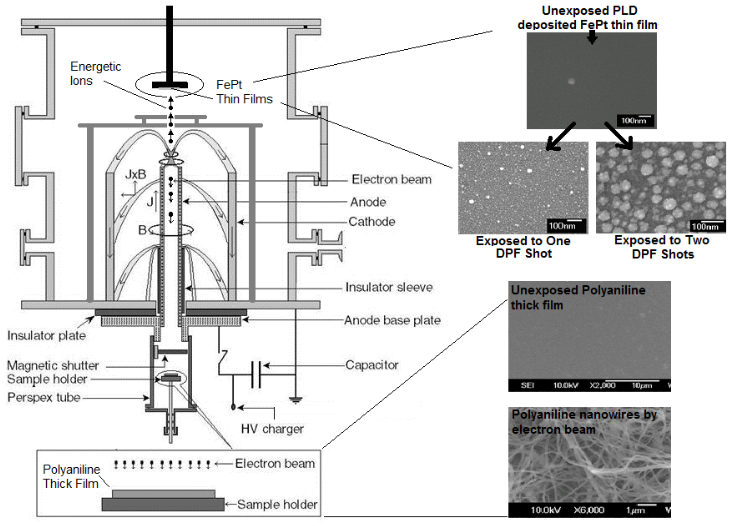
\includegraphics[width=0.6\textwidth]{figures/combined-schematic-of-dpf-device.png}
        \caption{\scriptsize The combined schematic of DPF device showing the exposure of FePt thin film to energetic ions in UNU/ICTP device in Singapore and PA thick film to energetic electrons in another DPF device in Guwahati, India. The images on the right show the changes in surface morphology to nanoparticles and nanowires after DPF exposure. \cite{rawat_2015_dense}}
        \label{fig:combined-schematic-of-dpf-device}
    \end{figure}
    \tiny{\cite{rawat_2015_dense} R. S. Rawat. Dense plasma focus - from alternative fusion source to versatile high energy density plasma source for plasma nanotechnology.}
\end{frame}

\begin{frame} {Mechanism of Nano-structuring}
    \begin{enumerate}
        \item Most of the H+ ions stop and deposit bulk of their energy in silicon substrate at the Bragg peak position as the thickness of FePt thin films was only about 67 or 100 nm.
        \item This results in heating of silicon substrate to very high temperature in a very short span of time.
        \item The thermal energy is then conducted to the FePt thin films and causes the diffusion of metal atoms either through the lattice or along grain boundaries.
        \item The diffusion releases the thermal expansion mismatch stresses between the silicon oxide layer of the silicon substrate surface and the PLD coated FePt thin film.
    \end{enumerate}
\end{frame}

\begin{frame} {Bottom-up Nanoscale Fabrication in DPF}
    \begin{itemize}
        \item The spherical nanoparticles (NPs) seen in Fig.\ref{fig:synthesis-of-nanostructures} (a-d) are the examples of 0-dim nanostructures synthesize in DPF devices.
        \item While NPs are visibly present over the entire substrate surface in Fig.\ref{fig:synthesis-of-nanostructures} (a and b), they are also present as the background in Fig.\ref{fig:synthesis-of-nanostructures} (c and d).
        \item Once background carpet of 0-dim NPs is formed on the substrate surface then higher dimensional nanostructures can grow on this NP carpet.
    \end{itemize}
\end{frame}

\begin{frame} {Synthesis of 0-, 1-, 2-, and 3-dimensional Nanostructures using DPF Device.}
    \begin{figure}
        \centering
        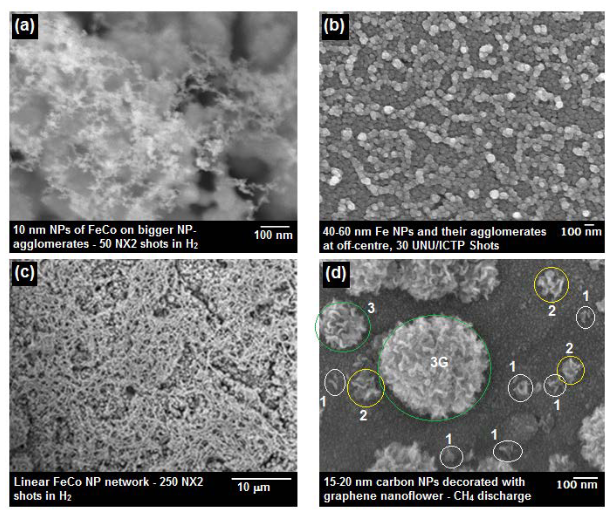
\includegraphics[width=0.6\textwidth]{figures/synthesis-of-0-1-2-3-dimensional-nanostructures.png}
        \caption{\scriptsize Synthesis of 0-, 1-, 2- and 3- dimensional nanostructures using DPF devices. \cite{rawat_2015_dense}}
        \label{fig:synthesis-of-nanostructures}
    \end{figure}
    \tiny{\cite{rawat_2015_dense} R. S. Rawat. Dense plasma focus - from alternative fusion source to versatile high energy density plasma source for plasma nanotechnology.}
\end{frame}